\def\year{2016}\relax
%File: formatting-instruction.tex
\documentclass[letterpaper]{article}
\usepackage{aaai16}
\usepackage{times}
\usepackage{helvet}
\usepackage{courier}

\usepackage[pdftex]{hyperref}
\usepackage{amsmath}
\usepackage{color}
\usepackage{textcomp}
\usepackage{booktabs}
\usepackage{ccicons}
\usepackage{todonotes}
\usepackage{amsfonts}

\frenchspacing
\setlength{\pdfpagewidth}{8.5in}
\setlength{\pdfpageheight}{11in}
\pdfinfo{
/Title (On Extensibility and Personalizability of Multi-Modal Trip Planning)
/Author (Put All Your Authors Here, Separated by Commas)}
\setcounter{secnumdepth}{0}  

\newcommand{\aux}{\mathit{aux}}
\newcommand{\dist}{\mathit{dist}}
\newcommand{\cA}{\mathcal{A}}
\newcommand{\cU}{\mathcal{U}}
\newcommand{\cP}{\mathcal{P}}
\newcommand{\tit}[1]{\textit{#1}}
\newcommand{\IFF}{\textit{iff}}
\newcommand{\IF}{\textit{if}}
\newcommand{\PCF}{\mathit{PCF}}
\newcommand{\walk}{\mathit{walk}}
\newcommand{\bike}{\mathit{bike}}
\newcommand{\car}{\mathit{car}}
\newcommand{\public}{\mathit{public}}
\newcommand{\taxi}{\mathit{taxi}}
\newcommand{\gas}{\mathit{gas}}
\newcommand{\wait}{\mathit{wait}}
\newcommand{\SUM}{\mathit{sum}}
\newcommand{\MAX}{\mathit{max}}
\newcommand{\MIN}{\mathit{min}}
\newcommand{\AVG}{\mathit{avg}}

\newcommand{\secref}[1]{Section~\ref{sec:#1}}
\newcommand{\figref}[1]{Figure~\ref{fig:#1}}
\newcommand{\tblref}[1]{Table~\ref{tbl:#1}}
\newcommand{\algref}[1]{Algorithm~\ref{alg:#1}}
\newcommand{\thmref}[1]{Theorem~\ref{thm:#1}}
\newcommand{\propref}[1]{Proposition~\ref{prop:#1}}
\newcommand{\corref}[1]{Corollary~\ref{cor:#1}}

 \begin{document}
% The file aaai.sty is the style file for AAAI Press 
% proceedings, working notes, and technical reports.
%
\title{On Extensibility and Personalizability of Multi-Modal Trip Planning}
\author{
	Xudong Liu\\
	Department of Computer Science\\
	University of Kentucky\\
	329 Rose Street\\
	Lexington, KY 40506\\
	USA
	\And
	PARC People\\
	Palo Alto Research Center\\
	3333 Coyote Hill Road\\
	Palo Alto, CA 94304\\
	USA
}
\maketitle
\begin{abstract}
	Trip planning is a practical task that has drawn
	extensive attention from the AI planning and scheduling community
	and the industrial/commercial sectors.
	In this paper, we consider the setting of the \tit{multi-modal}
	trip planning, where users can exploit different transportation
	modes, such as walking, biking, public transit, and taxi.
	In such a context, it would be of benefit if the
	user was able to extend the \tit{cost base}, including traveling time 
	and fare, of the planner, and to personalize the planner according
	to her own constraints and preferences.
	To this end, we designed and developed a hipergraph-based multi-modal
	trip planner that allows users to upload auxiliary cost metrics (e.g.,
	crime rates), to specify constraints as a theory in the 
	\tit{linear temporal logic}, and to express preferences as a 
	\tit{preferential cost function}.
\end{abstract}

\section{Introduction}
Trip planning, as an application of planning and scheduling,
has seen substansive implementations by researchers and
developers\cite{bast2015route}.
Some of the planning systems are \tit{multi-modal}; that is,
combining distinct transportation modes, the trip planners
compute optimal routes from sources to destinations.
This notion of ``optimality" generally refers to the computed routes
having minimal total time or total fare.

However, in the eyes of a user, it may be more faceted than just
``fastest" or ``cheapest."
For instance, for a college student who specifies that she will
only walk or take public transit in a trip from Palo Alto to
San Francisco, the computed plan is not necessarily the fastest
(e.g., taking a cab could be faster)
or the cheapest (e.g., walking all the way has no fare).
This happens when a user tells the planner her hard constraints,
called \tit{constraints}.  
The planner then needs to either satisfy the 
constraints in the search process or return failure because they are
over-restrictive.
Moreover, the user might want to further customize the planner by
describing soft constraints, called \tit{preferences}.
For example, an agent wants to travel from school to
downtown, and prefers biking to taking the bus.
Thus, a trip with more biking than bus may be considered better for
the agent than the one with more bus than biking.
In this case, the planner will need to accommodate user preferences
whenever possilbe in the search of optimal solutions.

Representing and reasoning about constraints and preferences are
fundamental to decision making in automated planning and scheduling
in artificial intelligence.
Son and Pontelli presented a declarative preference language, 
$\mathcal{PP}$, to represent ordinal preferences (e.g., basic desires,
atomic preferences and general preferences) between trajectories of 
a planning problem\cite{son2004planning}.
Bienvenu et al. proposed a first-order preference language, $\mathcal{LPP}$, 
extending $\mathcal{PP}$ by allowing the specification of quantified qualitative
preferences\cite{bienvenu2011specifying}.
Modesti and Sciomachen introduced an ad hoc utility function for weighing
the arcs both with their time and fare\cite{modesti1998utility}.
This relationship between time and fare in the setting of transportation
was studied, and economic models capturing the trade-off between the two
was presented\cite{antoniou2007methodology}.

However, relatively limited effort has been devoted to designing and
implementing real-world multi-modal trip planners that captures user
constraints and preferences over the \tit{cost base}, possibly
extended from the user with auxiliary \tit{cost metrics},
such as crime rates and pollution statistics.

Using a high-performance graph search
engine\cite{zhou2011dynamic}, we designed and implemented a 
multi-modal trip planner that uses pure
graph-search. This allows us to flexibly combine various modes
(e.g., walk, bike, car, public transit, and taxi) and 
declaratively change constraints and preferences. 
The planner allows the user
to upload \tit{new} mapping data over which to express
constraints and preferences.  For instance, a user might upload a map of crime
in the city, and ask the trip planner to avoid areas where crime is frequent.
Then, the planner takes constraints expressed in \tit{linear
temporal logic} to constrain the search space (e.g., never bike after
transit, and never walk through bad neighborhoods).
Finally, the planner uses a weighted sum, called \tit{preferential cost function}, 
over several cost metrics (e.g., time spend biking, fare on public transit, 
and overall crimes walking through) which can be re-weighted based
on different user preferences. 

%\begin{itemize}
%	\item What's the problem: personalized trip planning: find trips that
%	  are optimal in the eyes of a user, who doesn't care about mode or
%	  provider boundaries, and whose preferences may be more faceted than
%	  ``fastest'' or ``cheapest''.
%	\item Why is it hard: the computational complexity of searching
%	  combinations of multiple modes that can be combined freely is high
%	  (PSPACE-complete\cite{}) which is why existing trip planner exploit problem
%	  structure (such as only one mode per trip) and predefined
%	  preferences (optimization metrics)
%	\item How did we solve it: Using a high-performance graph search
%	  engine\cite{}, we implemented a multi-modal trip planner that uses pure
%	  graph-search. This allows us to flexibly combine various modes
%	  (e.g., car, train, cab, walk) and declarative change soft and hard
%	  constraints. The planner can take constraints expressed in linear
%	  temporal logic to constrain the search space (e.g., never bike after
%	  transit, i.e., I don't want to take my bike on the bus or train).
%	  The planner uses a weighted sum over several metrics (e.g., time
%	  overall, time spend on transit, cost) which can be re-weighted based
%	  on different user preferences. Finally the planner allows the user
%	  to upload {\em new} mapping data over which to express hard and/or
%	  soft constraints. For instance, a user might upload a map of crime
%	  in the city, and ask the trip planner to never walk at night through
%	  an area where crime is frequent.
%%	\item How did we evaluate the features and what are the results:
%%	  ceteris paribus experimentation setup on Amazon Mechanical 
%%		Turk (MTurk\footnote{\url{http://mturk.amazon.com}}) and results, 
%%		asking users to pick between two different trips, one being limited by the
%%	  capabilities of existing planners, and one exhibiting features only
%%	  available in our trip planner.
%\end{itemize}


\section{Extensibility}
%\begin{itemize}
%	\setlength\itemsep{1pt}
%	\item Explain in detail what extensibility means.
%	\item Describe the input.
%	\item Describe how we incorporate the auxiliary data into the planner.
%\end{itemize}
Allowing users to upload their own data sets of interests is an important
step towards customization of a trip planner.
We designed a framework where a user can upload auxiliary cost 
metric data (e.g., crime
statistics and pollution data) into the planner,
and the planner will compute an optimal route accordingly.

The user-created data are the auxiliary data that is represented as pairs
of latitude and longitude degrees.
To merge these lat-long pairs into the planner, we performed a neighborhood
search to calculate the total score of auxiliary data for each 
lat-long pair already in our planner.
It might be of strong interest to some user for our planning
system to take care of criminal statistics so that some level of safety
of the resulting routes is guaranteed.
For instance, a user traveling through the downtown area of San Francisco
around midnight may want to upload a data set of crimes (cf. \figref{sf_crime}), 
and express her constraints and preferences in hope of a preferred trip plan.

\begin{figure}[!ht]
  \centering
    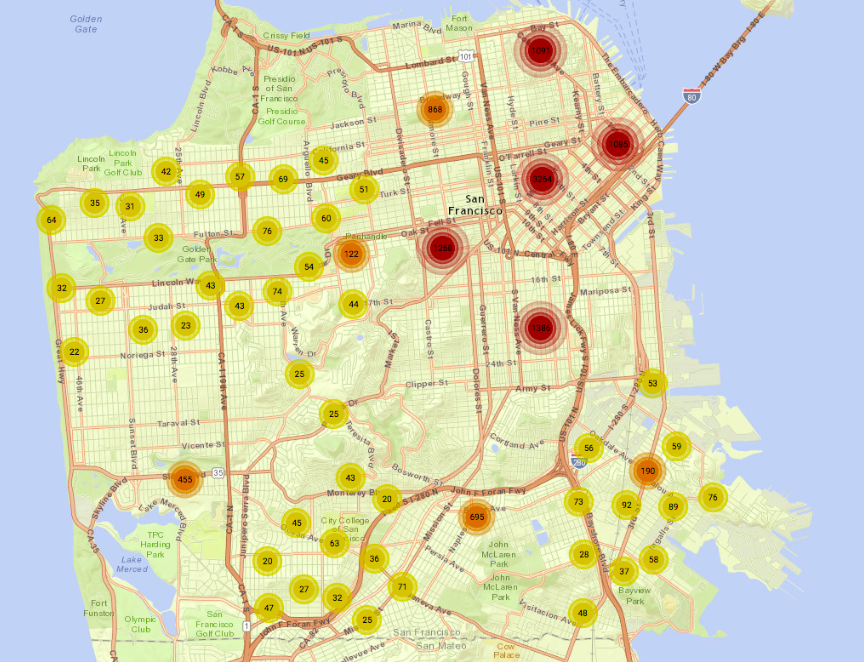
\includegraphics[width=0.4\textwidth]{figs/sub_sf_crime_July2015.png}
  \caption{Crime rates in San Francisco\label{fig:sf_crime}}
\end{figure}

Formally, let $\cU$ be the uploaded auxiliary dataset of lat-long pairs, 
$N=(x_N,y_N)$ a node in our planner and $r$ the effective radius.
We first compute the set $\cP \subseteq A$ of auxiliary points such that,
for every node $P \in \cP$, the Euclidean distance between $N$ and $P$
is within $r$.
Then, the score of auxiliary data for $N$ with respect to $\cP$ and $r$,
denoted by $S(N,\cP,r)$, is computed as follows.

\begin{equation*}
	S(N,\cP,r) = \sum_{\substack{P \in \cP}} 
		\Big(1 - \frac{\sqrt{(x_N-x_P)^2+(y_N-y_P)^2}}{r}\Big)
\end{equation*}

Now we turn to \figref{aux} for an instance to show how auxiliary data
are integrated into the graph using the equation above.
In \figref{aux}, we have the green nodes denoting the graph nodes, 
and the red nodes the new auxiliary nodes that represent locations
of criminal events.
For node $N$, there are three red nodes within its neighborhood of
radius of $r$; thus, we have $\cP=\{P_1,P_2,P_3\}$.
We assume $r$ is 100 feet, and the distances from $N$ to $P_1$,
$P_2$ and $P_3$ are 25, 80 and 90 feet, respectively.
Then, the crime score of $S(N,\cP,r)$ is $1.05$.

\begin{figure}[!ht]
  \centering
    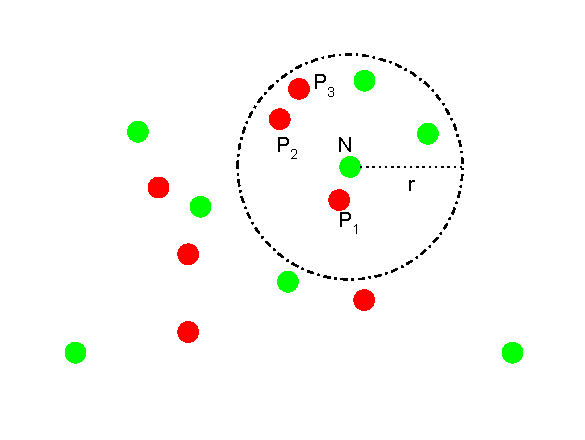
\includegraphics[width=0.4\textwidth]{figs/aux.pdf}
  \caption{Integrating uploaded data\label{fig:aux}}
\end{figure}


\section{Personalizability}
Personalizability consists of two aspects: constraints and preferences.
From the viewpoint of the planner,
constraints, also referred to as hard constraints, are statements that the planner
has to satisfy during the planning process; whereas preferences, also called
soft constraints, are specifications that the planner will need to optimize.
We formulated constraints using linear temporal logic (LTL) and preferences as
a preferential cost function (PCF), and implemented our planner leveraging the
widely-used graph search algorithm the A*.

\subsection{Constraints}
%\begin{itemize}
%	\setlength\itemsep{1pt}
%	\item Describe syntax and semantics of LTL in the setting of trip planning.
%	\begin{itemize}
%		\setlength\itemsep{0pt}
%		\item Specifically, we need to point out the ``after" temporal connective,
%					and we need to describe the semantics: what is a plan, why we can
%					eliminate actions and put them as state attributes instead, etc.
%	\end{itemize}
%\end{itemize}
As constraints in the setting of trip planning are often declarative and
temporal, our choice of LTL is straightforward.
We now give a brief review of linear temporal logic (LTL).
Let $f$ be a propositional formula over a finite set $L$ of Boolean variables.  
LTL formulas are defined recursively as follows.
\begin{equation}
	\varphi = f | \varphi_1 \land \varphi_2 | \varphi_1 \lor \varphi_2 | \neg \varphi | 
		\bigcirc \varphi |	\Box \varphi | \Diamond \varphi | \varphi_1 \cA \varphi_2
\end{equation}
Note that we have $\varphi_1 \cA \varphi_2$, and it means that
``$\varphi_2$ holds right after $\varphi_1$ holds."

A natural constraint in trip planning could be ``In this trip I will not drive a car 
after biking or taking the public transit."
In LTL, such constraint can be translated into an LTL formula
\begin{align*}
	\psi = ((M=b) \lor (M=p)) \,\cA\, (\Box (\neg (M=c))).
\end{align*}

As the actions in trip planning is limited to taking different transportation modes,
in our definition of the semantics of LTL
these actions are subsumed into the interpretations of $L$, or \tit{states}.
The semantics of LTL is defined with regard to trajectories of states. 
Let $\sigma$ be a trajectory of states $S_0,a_1,S_1,\ldots,a_n,S_n$, and
$\sigma[i]$ a suffix $S_i, a_{i+1}, S_{i+1}, \ldots,a_n,S_n$.  We have
\begin{align*}
	\sigma \models f \;\; &\IFF \;\; S_0 \models f,\\
	\sigma \models \varphi_1 \land \varphi_2 \;\; &\IFF \;\; \sigma \models \varphi_1 \; and \; \sigma \models \varphi_2,\\
	\sigma \models \varphi_1 \lor \varphi_2 \;\; &\IFF \;\; \sigma \models \varphi_1 \; or \; \sigma \models \varphi_2,\\
	\sigma \models \neg \varphi \;\; &\IFF \;\; \sigma \not \models \varphi,\\
	\sigma \models \bigcirc \varphi \;\; &\IFF \;\; \sigma[1] \models \varphi,\\
	\sigma \models \Box \varphi \;\; &\IFF \;\; \forall 0 \leq i \leq n (\sigma[i] \models \varphi),\\
	\sigma \models \Diamond \varphi \;\; &\IFF \;\; \exists 0 \leq i \leq n (\sigma[i] \models \varphi),\\
	\sigma \models \varphi_1 \cA \varphi_2 \;\; &\IFF \;\; \forall 0 \leq i < n (\IF \; \sigma[i] \models \varphi_1, \sigma[i+1] \models \varphi_2).
\end{align*}

For example, we are given an LTL constraint $\psi$ and three trajectories ($\sigma_1$, $\sigma_2$ and $\sigma_3$)
as shown in \figref{trjs}.
Clearly, we have $\sigma_1 \models \psi$ because, after public transit in $S_2$ and $S_3$, 
traveling by car has never been taken place.
Moreover, we have $\sigma_2 \not \models \psi$ because we have $M=c$ hold in $S_6$ and $S_7$
after having $M=p$ hold in $S_2$ and $S_5$.
Finally, we know $\sigma_3 \models \psi$, as the mode is always neither biking nor public transit.

\begin{figure}[!ht]
  \centering
    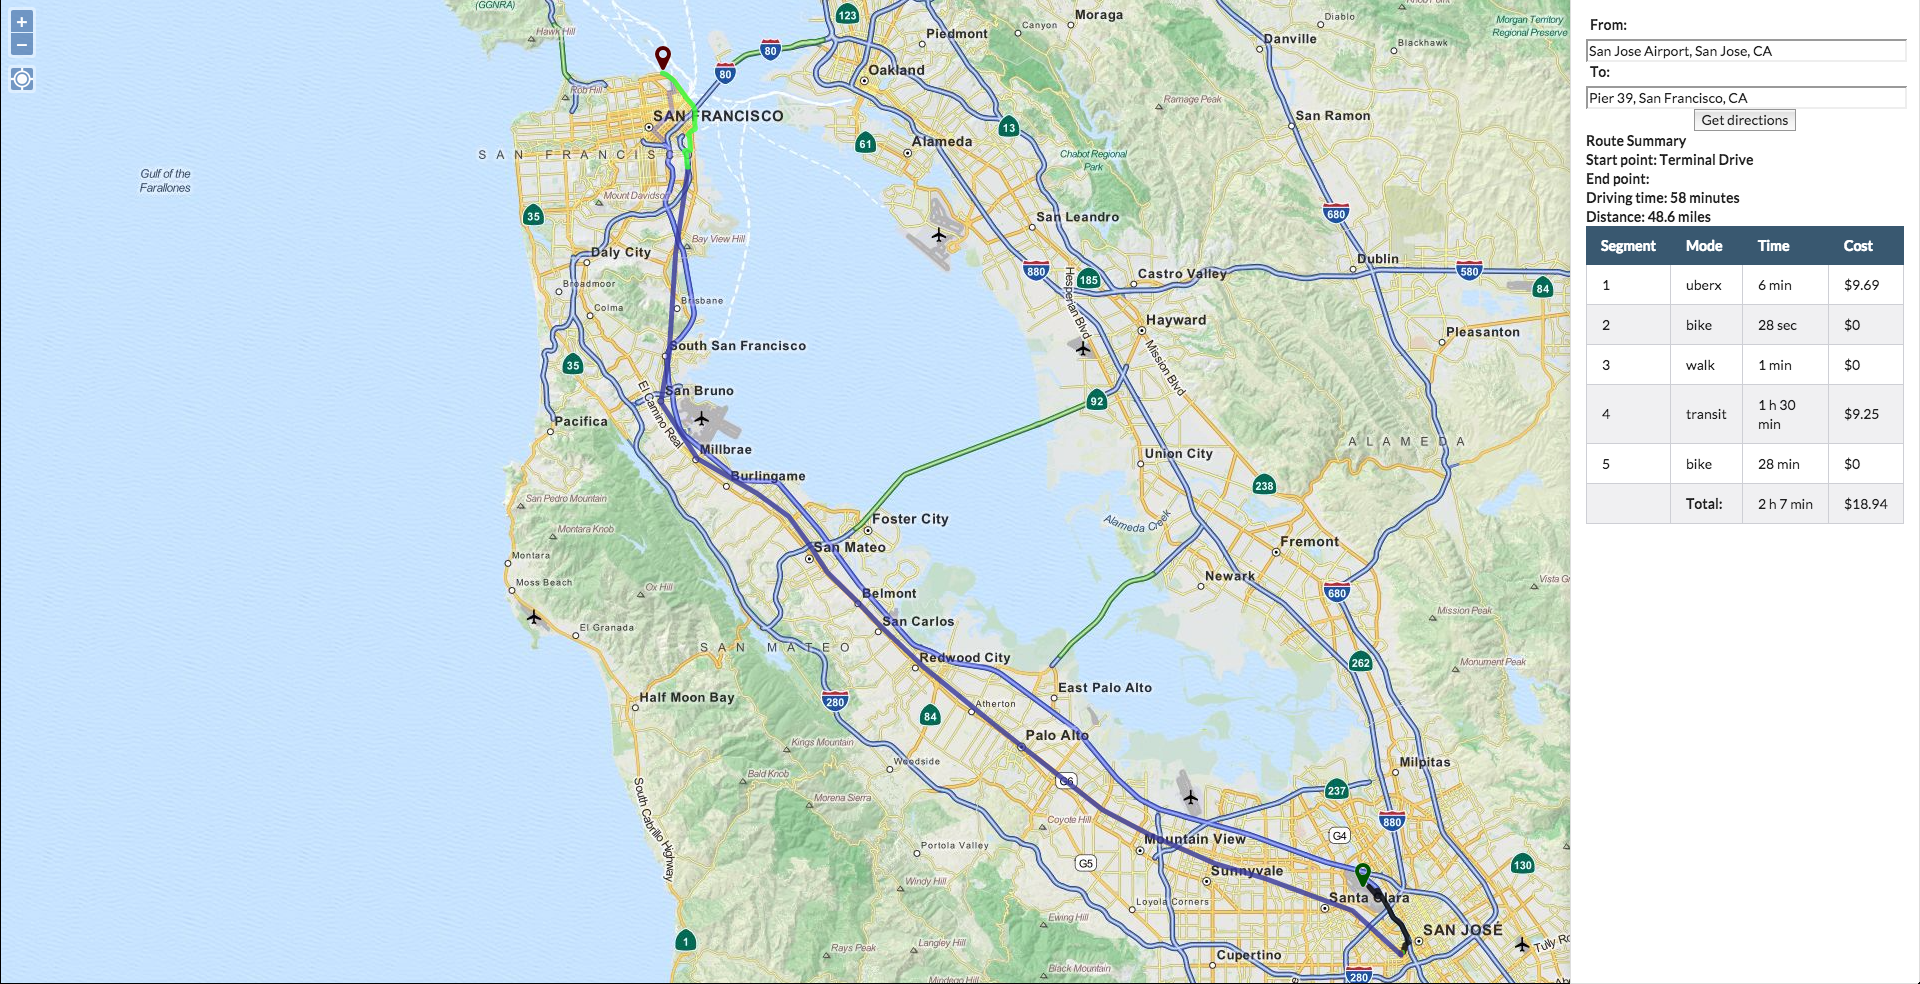
\includegraphics[width=0.5\textwidth]{figs/result1.png}
  \caption{State transition diagram\label{fig:trjs}}
\end{figure}


\subsection{Preferences}
%\begin{itemize}
%	\setlength\itemsep{1pt}
%	\item Describe our preferential cost function (PCF).
%	\begin{itemize}
%		\setlength\itemsep{0pt}
%		\item Describe why and how we break down time and money.
%		\item Describe why and how we design coefficients to these time and money pieces.
%		\item Describe why and how we design the two ratios: dollars per hour and dollars per aux.
%	\end{itemize}
%\end{itemize}

A state is described as a set of \tit{state variables}.
The state variables of a state $S$ include the transportation mode $M$ that led to $S$,
time spent $T$ so far per mode (e.g., $T_\bike$ for biking and $T_\public$ for
public transit), fare $D$ spent so far per mode (e.g., $D_\gas$ for driving and
$D_\taxi$ for taking a cab), and variables related to the auxiliary data once uploaded.
These extra data related variables are metrics such as the sum ($A_\SUM$),
the maximum ($A_\MAX)$, the minimum ($A_\MIN$), and the average ($A_\AVG$) data along the path.

We focused on weighted functions over state variables and
designed the cost function, called preferential cost function (PCF), that guides the
graph-based search engine in our trip planner as follows.
\begin{equation}
	\begin{aligned}
		\PCF(S) =& \beta_1 * (\alpha_1 \cdot T_\walk + \alpha_2 \cdot T_\wait + \ldots) \\
								&+ (D_\gas + D_\public + \ldots) \\
								&+ \beta_2 * (A_\SUM + \ldots),
	\end{aligned}
\end{equation}
where $\alpha_i$ are real numbers representing the relations among different time pieces,
and $\beta_1$ ($\beta_2$) is the ratio that essentially describes how much in dollars a user would pay to
save an hour (an auxiliary data, respectively).

\subsubsection{Preference Elicitation}
To gather these coefficients ($\alpha_i$ and $\beta_i$) in our $\PCF$, we designed interface to
elicit these numbers from the user.

\subsection{Reasoning with Constraints and Preferences}
%\begin{itemize}
%	\setlength\itemsep{1pt}
%	\item Describe why and how we integrate constraints and preferences into A*.
%\end{itemize}

\begin{figure}[!ht]
  \centering
    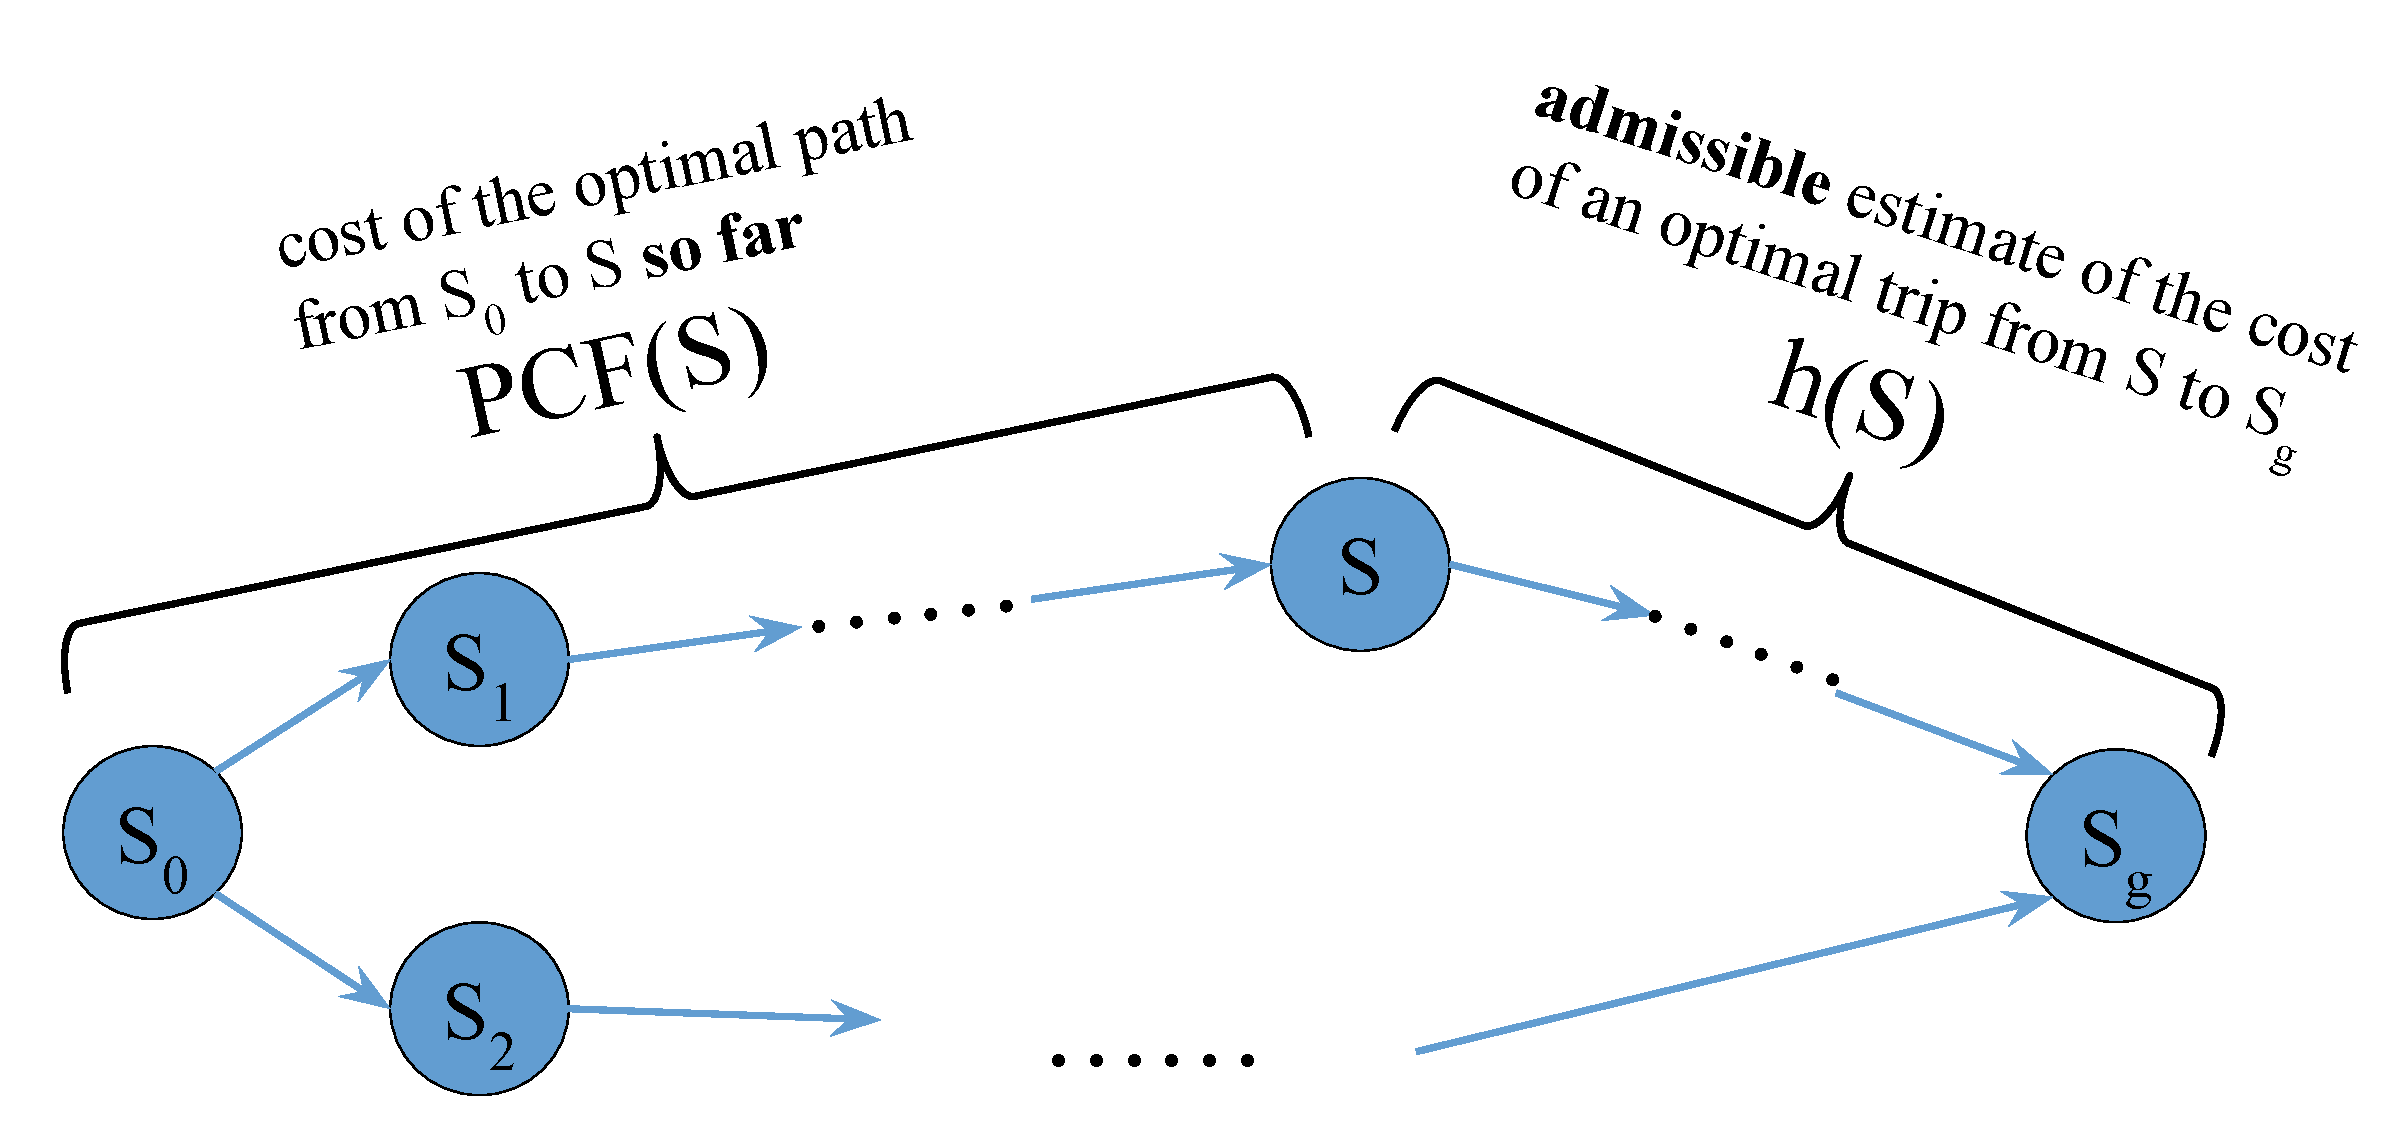
\includegraphics[width=0.4\textwidth]{figs/Astar.pdf}
  \caption{Adjusted A*\label{fig:astar}}
\end{figure}

We leveraged the widely-used A* search algorithm on top of our high-performance graph search
engine (cf. \figref{astar}).  The A* algorithm incorporates the following cost function.
\begin{equation}
	f(S) = g(S) + h(S),
\end{equation}
where $g(S)$ is the cost of an optimal trip from the initial state to $S$, and
$h(S)$ is an admissible estimate of the cost of an optimal trip from $S$ to goal.

To prune the search space, we check satisfiability of the temporal constraints in LTL
at expansion of the search tree.
To guide the search engine, we set $g(S)=\PCF(S)$ and $h(S)$ the minimum estimate among
all available modes in $S$.

%\section{User Study}
%\begin{itemize}
%	\setlength\itemsep{1pt}
%	\item Describe the set up of our experiments on AMT and explain why: because we want to evaluate the
%				feasibility of the three features.
%	\item Describe the results.
%\end{itemize}
\section{Implementation and Results}
%\begin{itemize}
%	\setlength\itemsep{1pt}
%	\item Describe the system structure.
%	\item Describe the input to the system.
%	\item Describe the output from the system.
%\end{itemize}

\subsection{System Architecture}
\begin{figure*}[!ht]
  \centering
    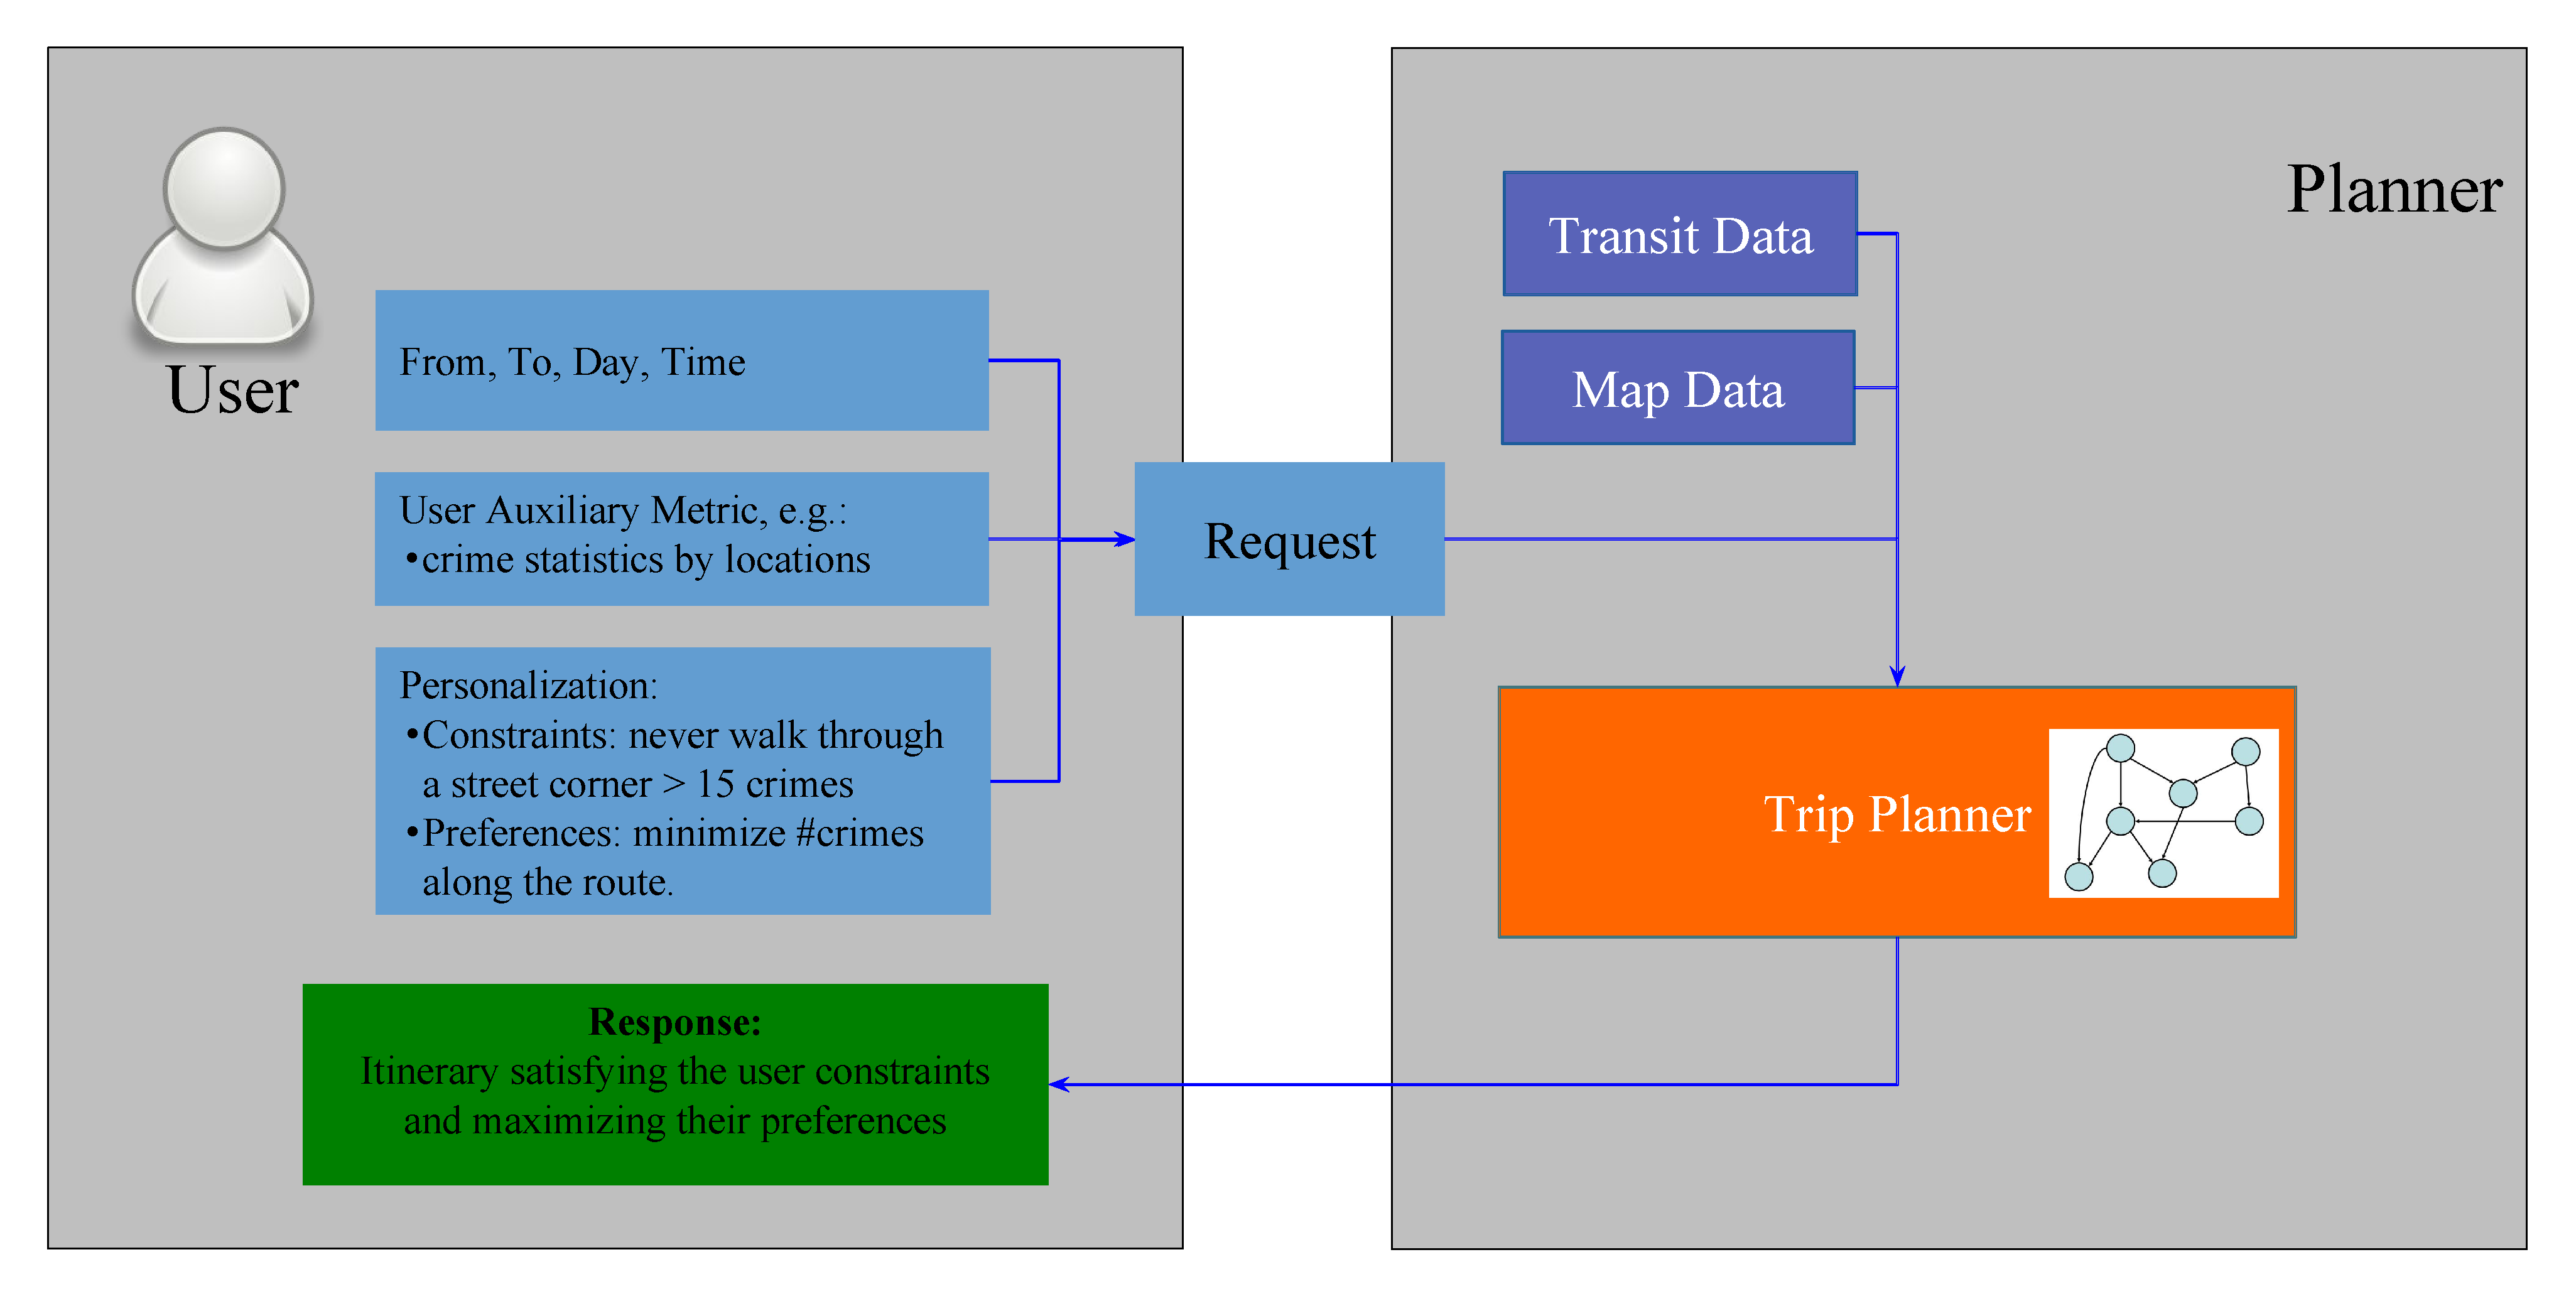
\includegraphics[width=0.8\textwidth]{figs/system.pdf}
  \caption{System Overview\label{fig:system}}
\end{figure*}

\subsection{Results}
First, we show resulting route for Alice in \figref{alice}.
\begin{figure}[!ht]
  \centering
    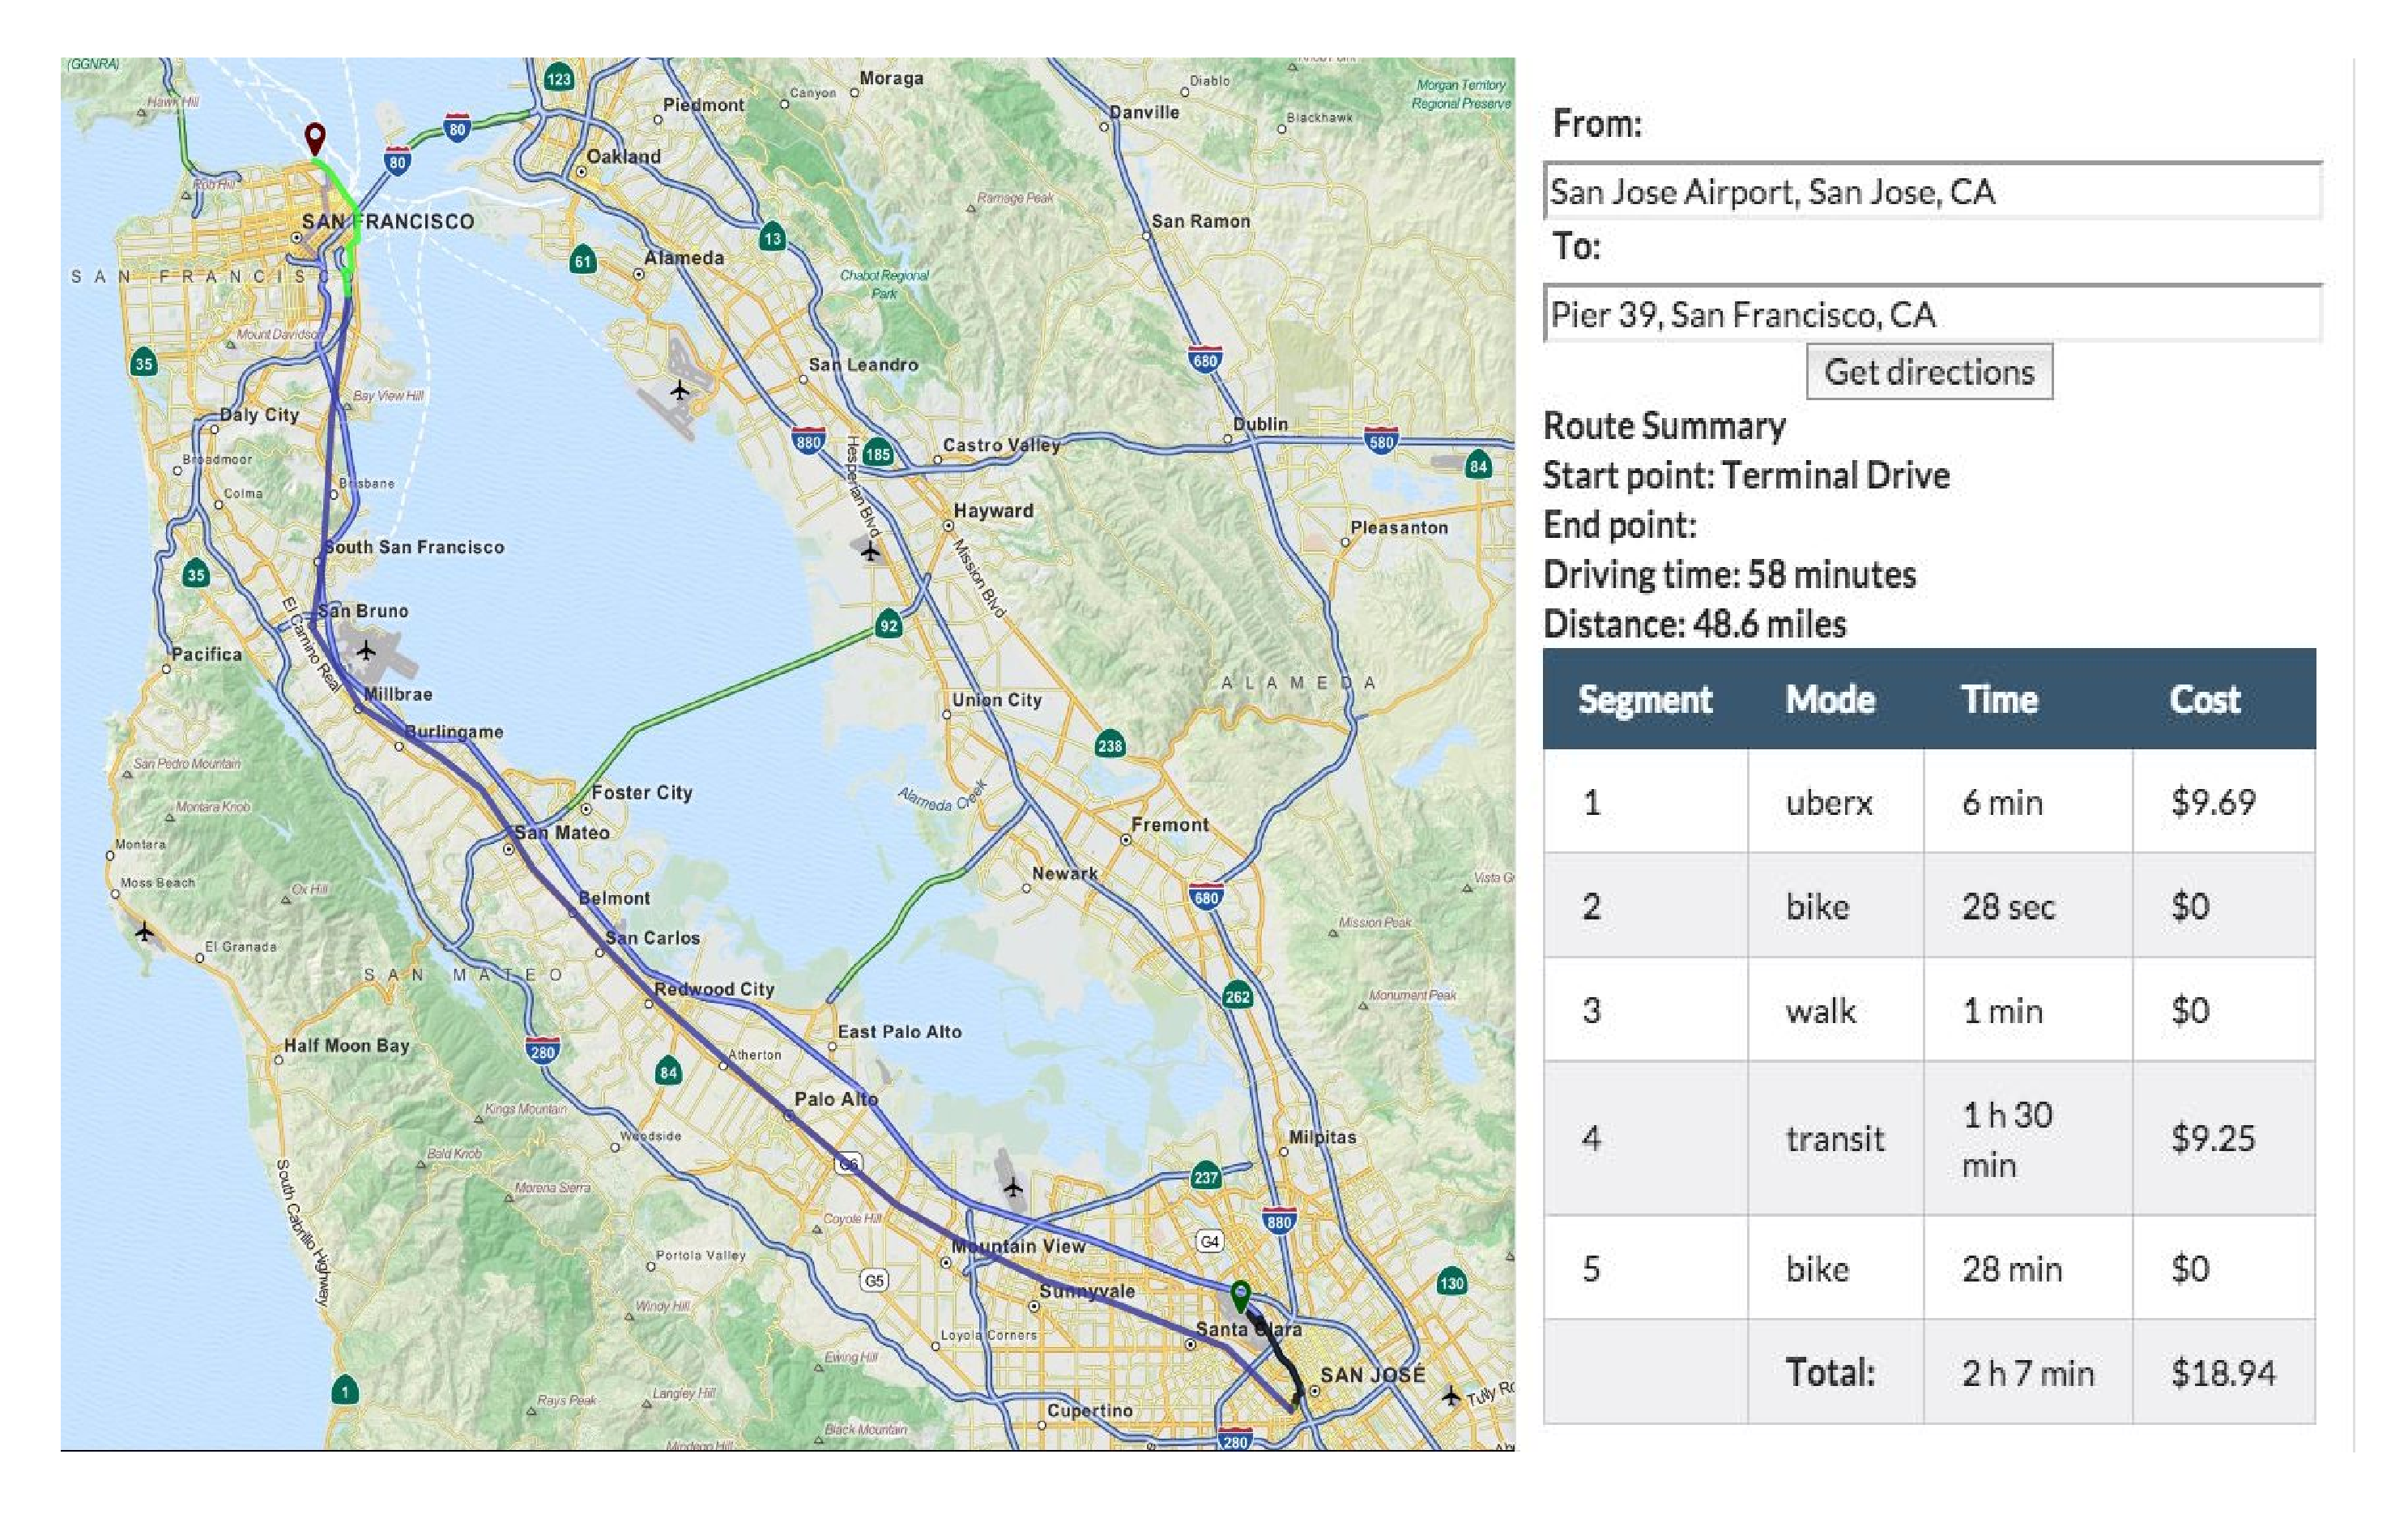
\includegraphics[width=0.5\textwidth]{figs/result_Alice.pdf}
  \caption{Resulting route for Alice\label{fig:alice}}
\end{figure}

Second, we show resulting route for Bob in \figref{bob}.
\begin{figure}[!ht]
  \centering
    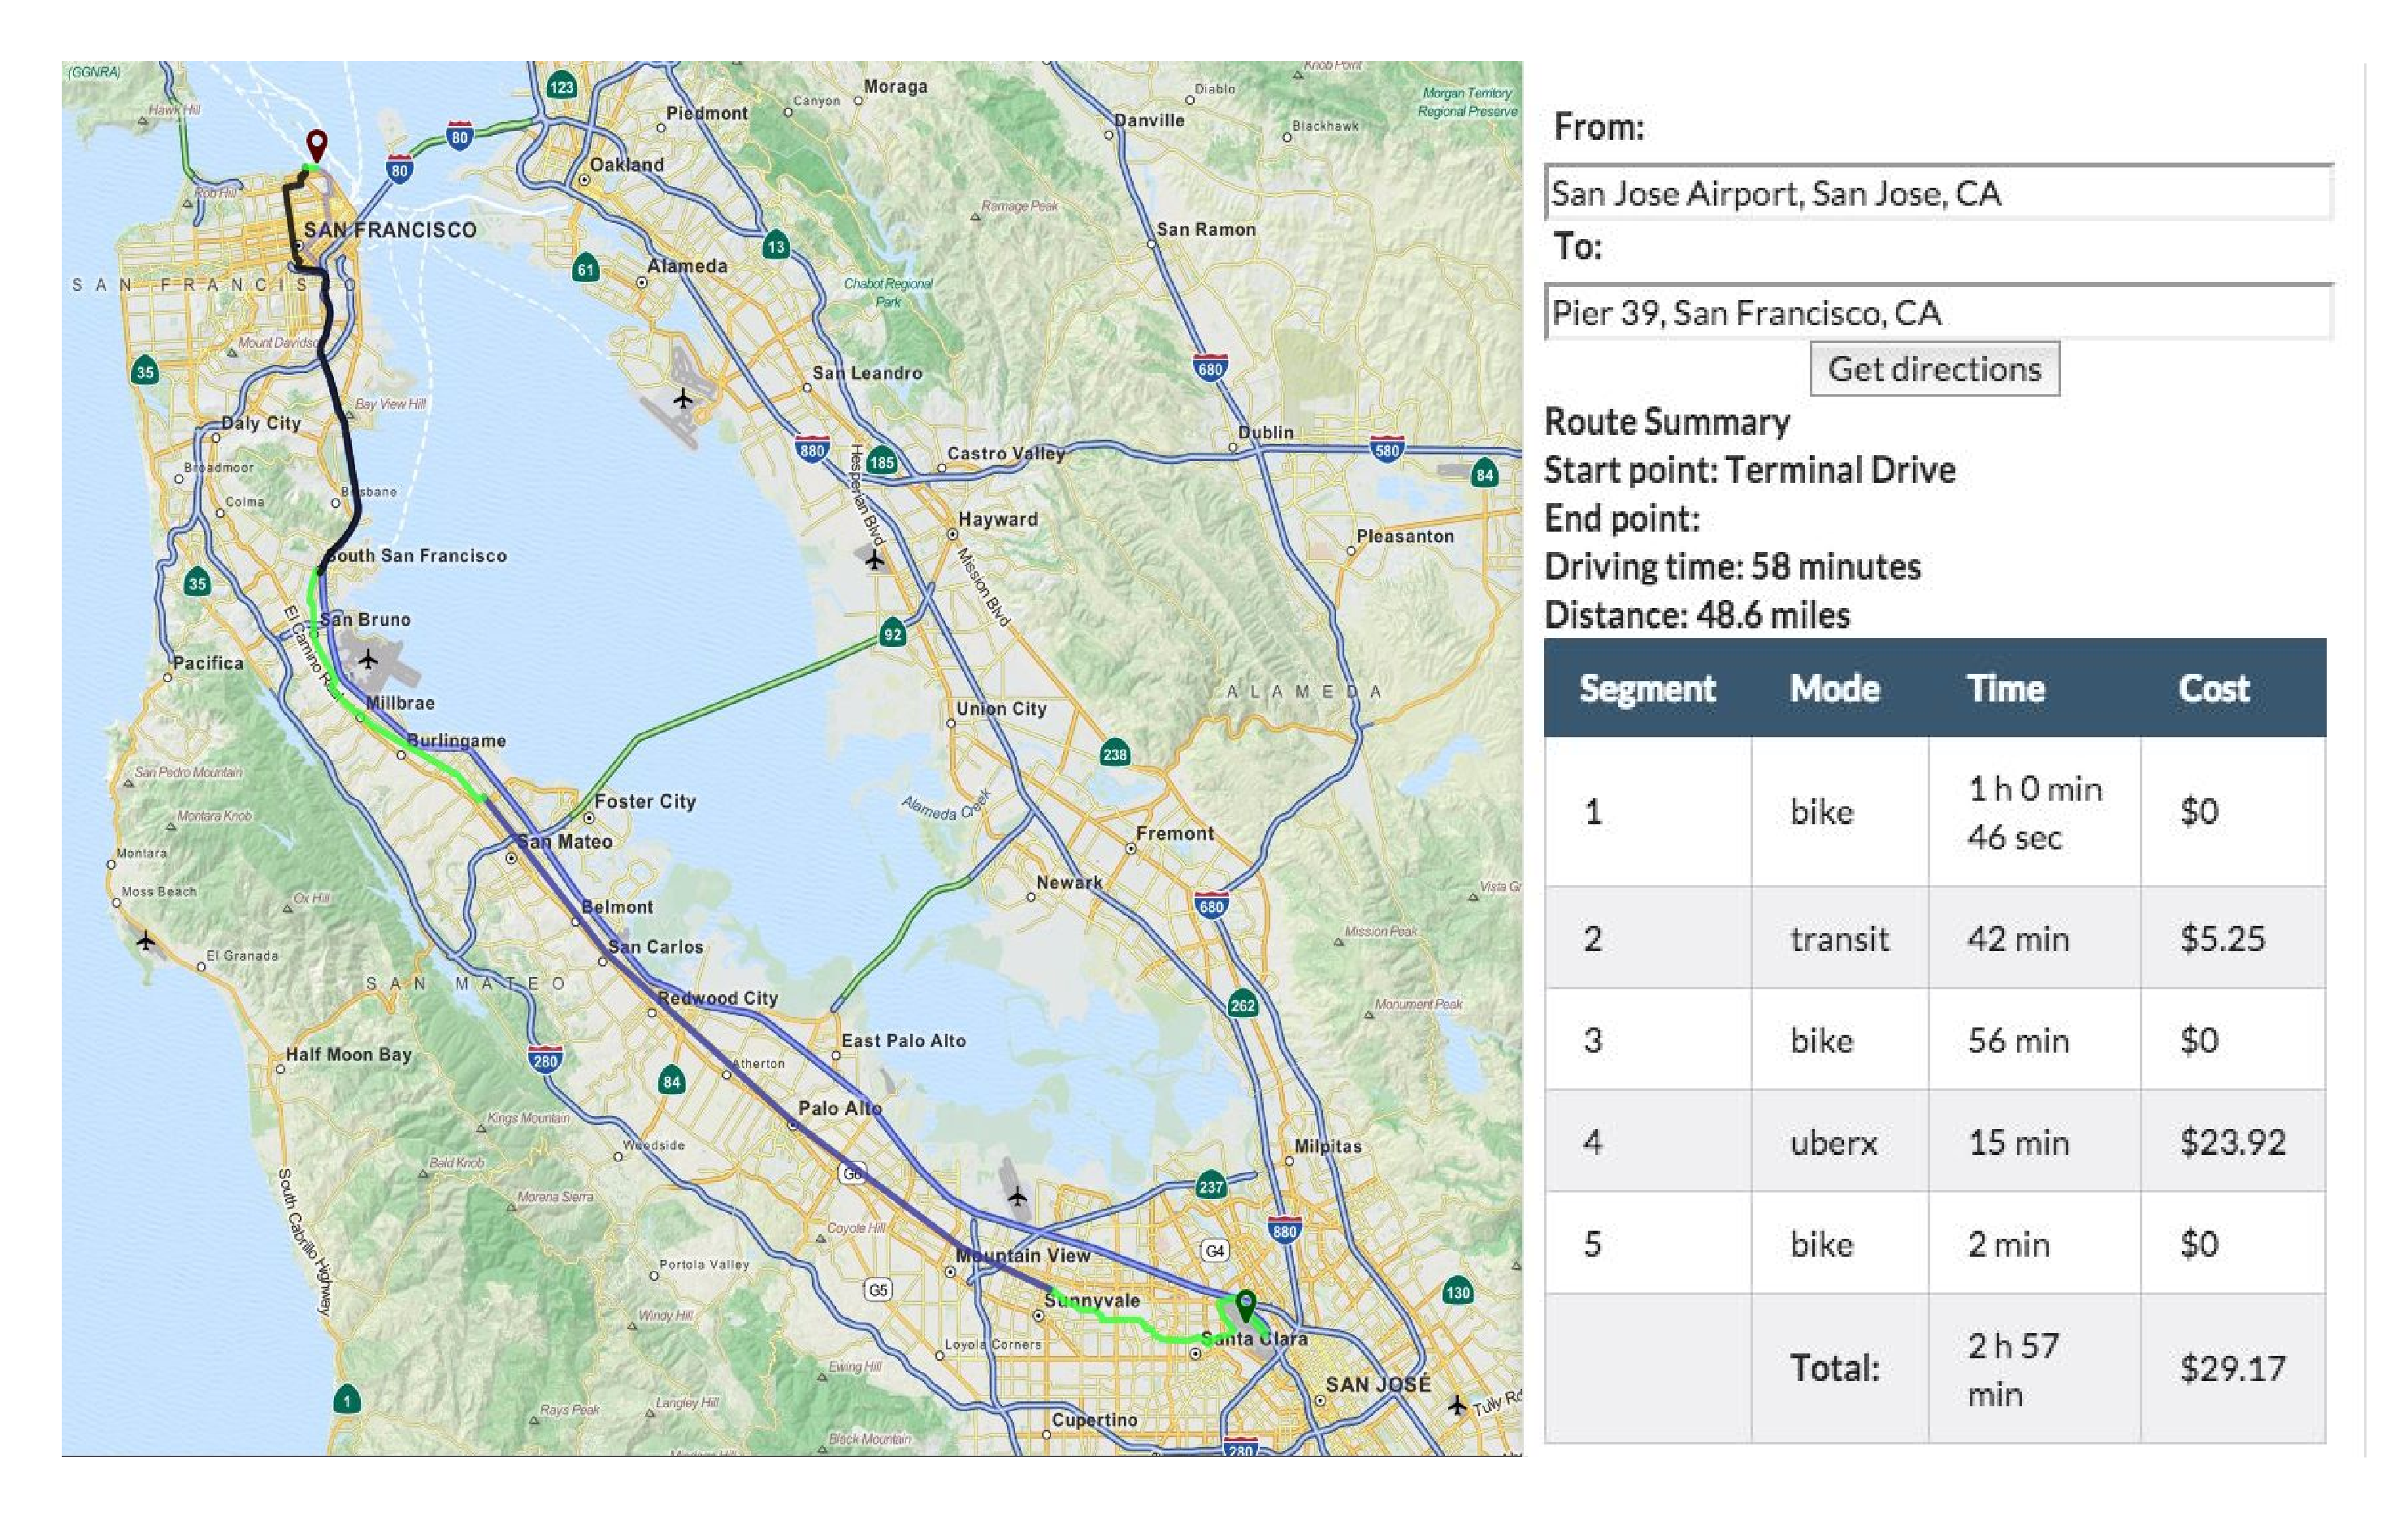
\includegraphics[width=0.5\textwidth]{figs/result_Bob.pdf}
  \caption{Resulting route for Bob\label{fig:bob}}
\end{figure}

Third, we show resulting route for Cal in \figref{cal}.
\begin{figure}[!ht]
  \centering
    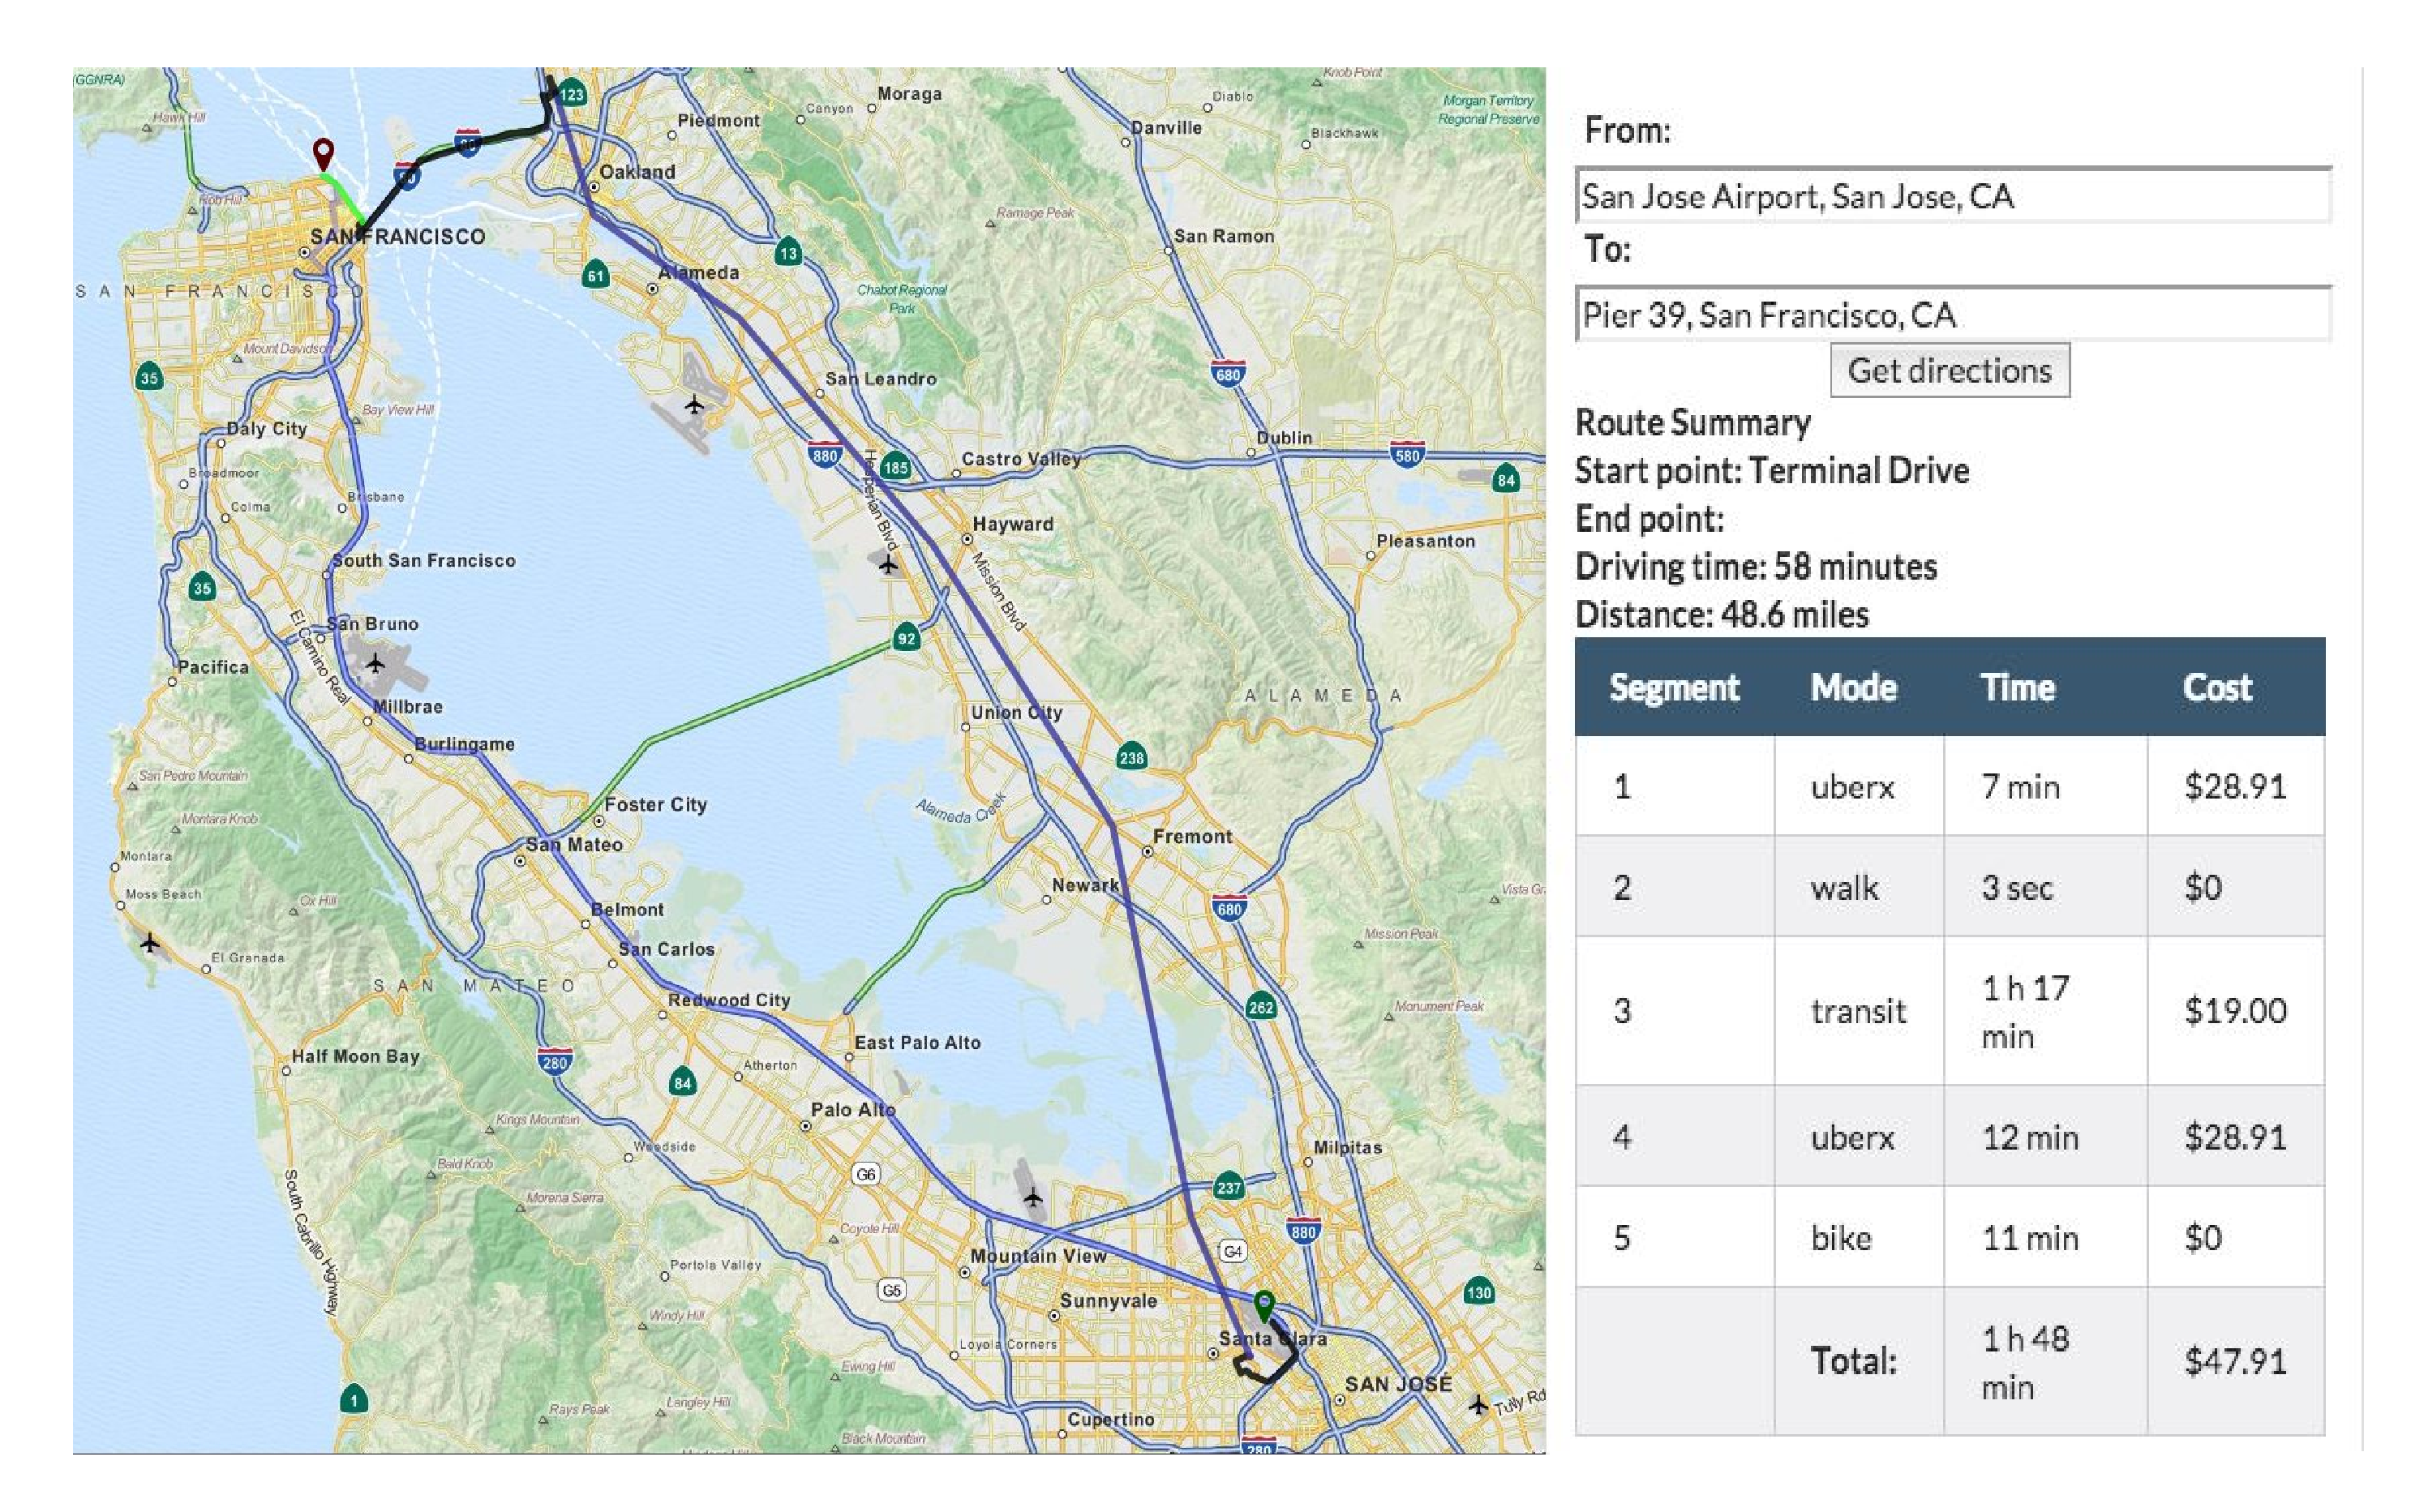
\includegraphics[width=0.5\textwidth]{figs/result_Cal.pdf}
  \caption{Resulting route for Cal\label{fig:cal}}
\end{figure}



\section{Conclusion and Future Work}


\bibliographystyle{aaai}
\bibliography{refs}



\end{document}
